%%%%%%%%%%%%%%%%%%%%%%%%%%%%%%%%%%%%%%%%%%%%%%%%%%%%%%%%%%%%%%%%%%%%%%%%%%%%%%%
%% Application of AL to stable polymorph discovery in the iridium-oxide space
%%
%%
%%%%%%%%%%%%%%%%%%%%%%%%%%%%%%%%%%%%%%%%%%%%%%%%%%%%%%%%%%%%%%%%%%%%%%%%%%%%%%%


% ################################# Paragraph #################################
% %%%%%%%%%%%%%%%%%%%%%%%%%%%%%%%%%%%%%%%%%%%%%%%%%%%%%%%%%%%%%%%%%%%%%%%%%%%%%
% TEMP
% %%%%%%%%%%%%%%%%%%%%%%%%%%%%%%%%%%%%%%%%%%%%%%%%%%%%%%%%%%%%%%%%%%%%%%%%%%%%%
% IrO2 Structure Analysis
- Describe relevant features
  - Physical intuition?
- Describe convex hull plot (energy vs. Ir-O distance), computed amorphous phase to define synthesizability
- While only 2 \ce{IrO_2} in MP/OQMD, we can compare our structures to other computed \ce{IrO_2} not in open databases.


% TEMP #COMBAK Remove dummy citation after real ones start coming in
This is a citation example \cite{dummy9999}.

% | - Figure | IrO2 Convergence Plot
\begin{figure*}
\centering
\makebox[\textwidth][c]{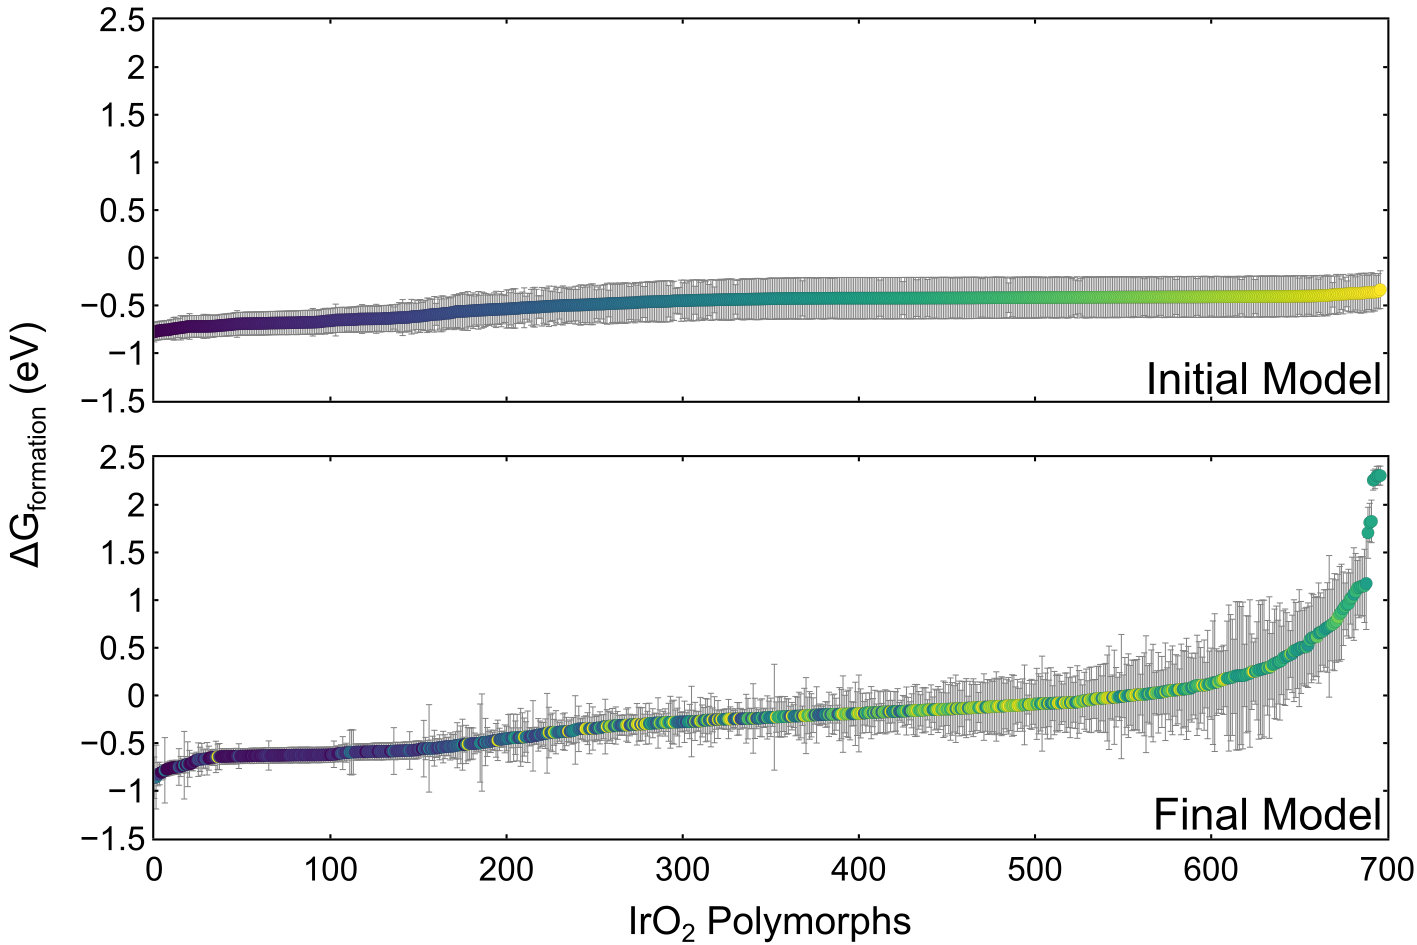
\includegraphics
  {02_figures/ml_convergence_plots/00_master__iro2-ml-conv_v1__200dpi__0__outplot.png}
  % {02_figures/ml_convergence_plots/iro2_ml_conv.png}
  }
\caption{\label{fig:convergence_plot_iro2_0}
% #COMBAK Subscript IrO2
Gaussian process machine learning models trained initially on (a) publicly available DFT data for IrO2 and (b) all of the acquired DFT calculations from the active learning algorithm.
See SI for additional panels at intermediate iterations of the active learning algorithm.
The Gibbs formation energy (either DFT derived or predicted from the GP model) and associated GP estimated error (2 sigmas or something TEMP) is plotted for each polymorph in the IrO2 candidate space.
The data points in each subset are ordered from most to least stable (lowest to largest DE formation).
The individual markers are colored based on their ordering in the final converged GP model.
Acquired structures are identified by their red borders and slightly larger size.
The insets show the most stable TEMP structures, where several well known crystal structures are labeled.
}
\end{figure*}
% __|


% ################################# Paragraph #################################
% %%%%%%%%%%%%%%%%%%%%%%%%%%%%%%%%%%%%%%%%%%%%%%%%%%%%%%%%%%%%%%%%%%%%%%%%%%%%%
% TEMP
% %%%%%%%%%%%%%%%%%%%%%%%%%%%%%%%%%%%%%%%%%%%%%%%%%%%%%%%%%%%%%%%%%%%%%%%%%%%%%
% AB3 Structures and Training
- XYZ unique AB3 Structures, 259 unique prototypes.  Substitute Ir and O, expand to minimum Ir-O distance > XYZ
- followed same procedure as in 3.1, Training Set of 35 structures, 8 of which are \ce{IrO_3}
- Describe initial training and training after first 10 DFT structures

% ################################# Paragraph #################################
% %%%%%%%%%%%%%%%%%%%%%%%%%%%%%%%%%%%%%%%%%%%%%%%%%%%%%%%%%%%%%%%%%%%%%%%%%%%%%
% TEMP
% %%%%%%%%%%%%%%%%%%%%%%%%%%%%%%%%%%%%%%%%%%%%%%%%%%%%%%%%%%%%%%%%%%%%%%%%%%%%%
% P2 Analysis of \ce{IrO_3} Structures
% #COMBAK Change alpha to actual greek symbol
- Describe convex hull, classes of structures (\ce{$\alpha$-AlF3} like, rutile like, and layered, should be segregated in hull plot)
- briefly describe structures within each class, cite in literature where appropriate


% | - Figure | IrO3 Convergence Plot
\begin{figure*}
\centering
\makebox[\textwidth][c]{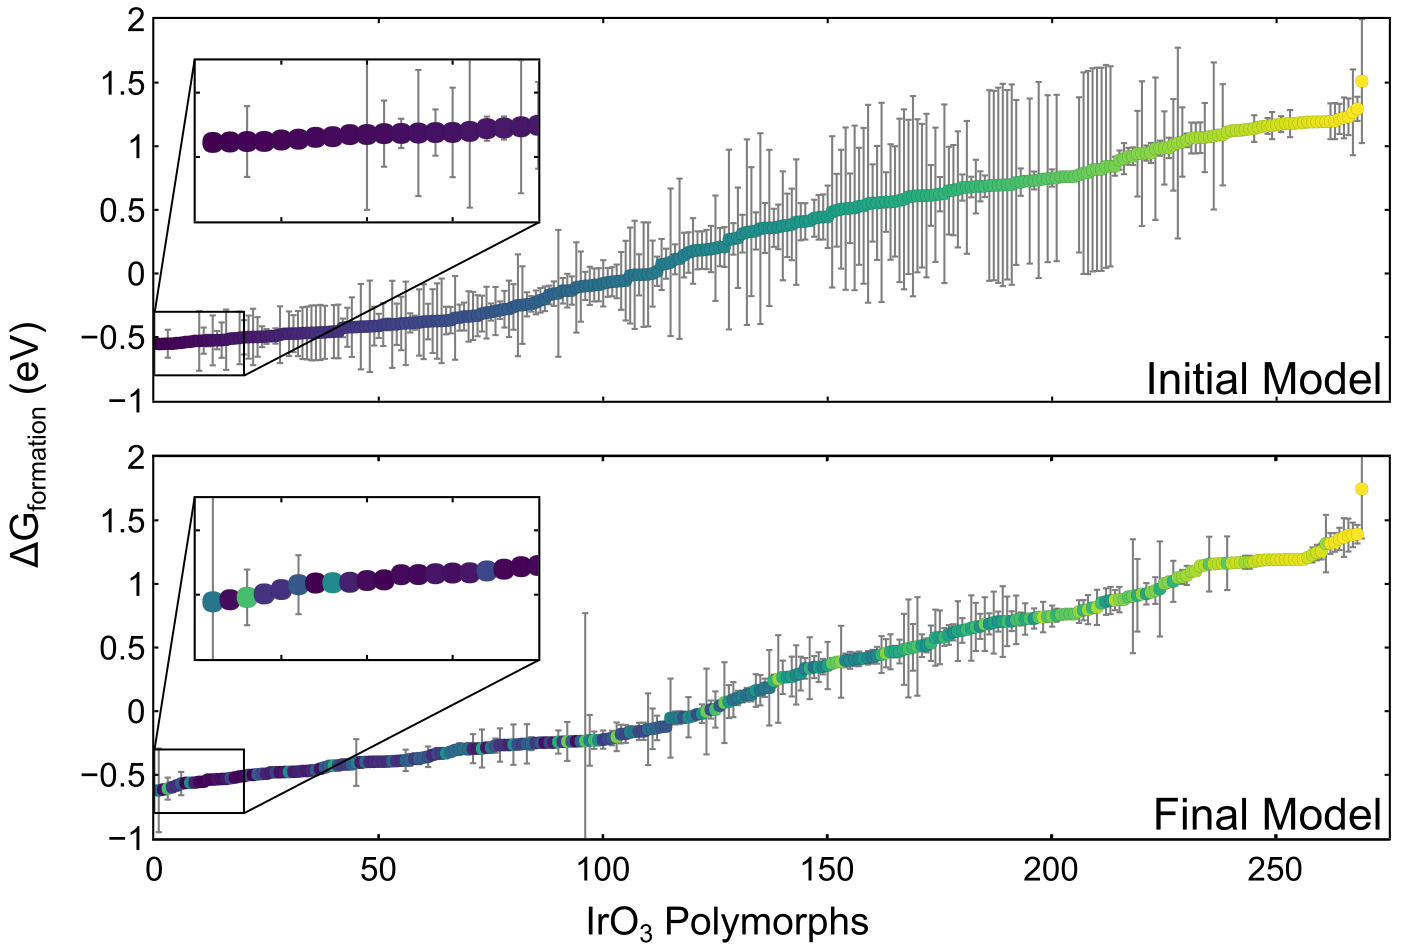
\includegraphics
{02_figures/ml_convergence_plots/00_master__iro3-ml-conv_v6__200dpi__0__outplot.png}
% {02_figures/ml_convergence_plots/iro3_ml_conv.png}
}
\caption{\label{fig:convergence_plot_iro3_0}
TEMP.
}
\end{figure*}
% __|
